\section{Results}
\label{sec:results}

All comparisons use the 50 Fairall~9 spectra and the 18 EG\,21 spectra. ``BANZAI'' denotes the archive products of
\banzai{}~1.0.1; ``this work'' denotes the full recalibration (re-extraction with the new fringe correction and sky,
arc refit, telluric zero point, and the template$\times$correction flux calibration with the median of the EG\,21
sensitivities, whose grey level is set by the clearest half of the standards). Table~\ref{tab:summary} collects the main numbers.

\begin{table*}
\centering
\caption{Summary of the quality metrics. Scatters are robust (1.4826 times the median absolute deviation) over the
50 Fairall~9 spectra unless stated otherwise. Small-scale scatter: rms over the 50 spectra of the ratio of each
(normalised) spectrum to the median spectrum after removing a 200\,\AA{} running median. Fringe metric: rms of the
ratio of 25\,\AA{} to 200\,\AA{} running medians in the telluric-free windows 7750--8050 and 8450--8900\,\AA.}
\label{tab:summary}
\begin{tabular}{lccc}
\toprule
Metric & BANZAI 1.0.1 & this work (optimal) & this work (boxcar) \\
\midrule
\multicolumn{4}{l}{\textit{Wavelengths (narrow lines at $z=0.047016$; median offset and scatter, \kms)}}\\
{[O\,{\sc iii}]\,5007, blue order} & \OIIIbOld & \multicolumn{2}{c}{\OIIIbNew} \\
{[O\,{\sc iii}]\,5007, red order} & \OIIIrOld & \multicolumn{2}{c}{\OIIIrNew} \\
{[O\,{\sc iii}]\,4959, blue order} & \OIIIfourOld & \multicolumn{2}{c}{\OIIIfourNew} \\
{[Ne\,{\sc iii}]\,3869, blue order} & \NeIIIOld & \multicolumn{2}{c}{\NeIIINew} \\
{[O\,{\sc i}]\,6300, red order} & \OIOld & \multicolumn{2}{c}{\OINew} \\
Ca\,{\sc ii}\,K (host), blue order & \CaKOld & \multicolumn{2}{c}{\CaKNew} \\
\midrule
\multicolumn{4}{l}{\textit{Red-order fringing and artefacts}}\\
Fringe metric (median of 50, per cent) & \FrOld & \FrNewOpt & \FrNewBox \\
Fringe in the median of 50 spectra, 7300--9500\,\AA{} (per cent) & \FrMedOld & \FrMedNewOpt & \FrMedNewBox \\
$>8\sigma$ spikes at 4600--5800\,\AA{} (median / maximum) & \SpOld & \SpNewOpt & \SpNewBox \\
\midrule
\multicolumn{4}{l}{\textit{Small-scale scatter between spectra (per cent)}}\\
blue 3500--4000\,\AA & \SSbaOld & \SSbaOpt & \SSbaBox \\
blue 4000--4600\,\AA & \SSbbOld & \SSbbOpt & \SSbbBox \\
blue 4600--5200\,\AA & \SSbcOld & \SSbcOpt & \SSbcBox \\
blue 5200--5700\,\AA & \SSbdOld & \SSbdOpt & \SSbdBox \\
red 5000--6000\,\AA & \SSraOld & \SSraOpt & \SSraBox \\
red 6000--6800\,\AA & \SSrbOld & \SSrbOpt & \SSrbBox \\
red 7000--7500\,\AA & \SSrcOld & \SSrcOpt & \SSrcBox \\
red 7700--8500\,\AA & \SSrdOld & \SSrdOpt & \SSrdBox \\
red 8500--9500\,\AA & \SSreOld & \SSreOpt & \SSreBox \\
\midrule
\multicolumn{4}{l}{\textit{Flux consistency (per cent)}}\\
{[O\,{\sc iii}]\,5007 flux scatter, blue order} & \FOIIIbOld & \FOIIIbOpt & \FOIIIbBox \\
{[O\,{\sc iii}]\,5007 flux scatter, red order} & \FOIIIrOld & \FOIIIrOpt & \FOIIIrBox \\
red/blue [O\,{\sc iii}] flux ratio scatter & \FRBOld & \FRBOpt & \FRBBox \\
EG\,21 shape vs CTIO, blue (18 nights) & \CLbOld & \multicolumn{2}{c}{\CLbNew} \\
EG\,21 shape vs CTIO, red (18 nights) & \CLrOld & \multicolumn{2}{c}{\CLrNew} \\
EG\,21 red fringe-scale rms (median of 18) & \EGfrOld & \multicolumn{2}{c}{\EGfrNew} \\
\bottomrule
\end{tabular}
\end{table*}

\subsection{Wavelength calibration}
\label{sec:results_wl}
Fig.~\ref{fig:zeropoint} shows the wide-slit problem in the archive products: the blue-order [O\,{\sc iii}] position
of Fairall~9 scatters by 2.8\,\AA{} rms from exposure to exposure, whereas the 5577\,\AA{} sky line on the same frames
scatters by 0.4\,\AA; the object's shift correlates with the telluric A band measured in the red order ($r=0.99$ in
pixels) and not with the sky lines. The red and blue orders disagree on [O\,{\sc iii}] by $-5.9\pm3.0$\,\AA.

After the arc refit and the telluric zero point (Fig.~\ref{fig:redshift}, Table~\ref{tab:summary}) the nuclear lines
agree from exposure to exposure to 20--40\,\kms{} in both orders and the two orders agree with each other to
$\approx10$\,\kms. Applying each night's own arc fit instead of the median correction increases the red--blue scatter
from 0.6 to 1.0\,\AA, confirming that the arc solution's shape is stable and the per-night fit only adds noise. Two
further tests support the method: (i) before correction, the shifts of [O\,{\sc iii}] and [Ne\,{\sc iii}] follow the
applied zero point with slopes 0.94 and 0.96, whereas the host-galaxy Ca\,{\sc ii}\,K absorption follows it with slope
0.17 -- the host is extended and fills the slit like the sky, and the correction is appropriate for the nuclear light
that RM measures (a caveat for host-starlight decomposition); (ii) the cleaner red order now yields [O\,{\sc i}]\,6300 in
\OIN{} of the 50 spectra at \OIvel\,\kms, while [O\,{\sc iii}] sits at \OIIIvel\,\kms, i.e. $\approx150$\,\kms{} to the
blue of [O\,{\sc i}], a typical [O\,{\sc iii}] outflow signature; this bounds the absolute zero-point error at
$\approx2$\,\AA.

\subsection{Fringing, sky and extraction}
\label{sec:results_fringe}
Fig.~\ref{fig:edge} shows the frame region where the shifted lamp flat had destroyed the data; the stripes are gone
and the largest number of spikes in a spectrum drops from \SpMaxOld{} to \SpMaxNew. Fig.~\ref{fig:residuals} shows the
2-d residuals: in the bright-moon frame the robust rms of the normalised residuals at 7000--9500\,\AA{} drops from
1.70 to 1.44 in the sky rows and from 1.83 to 1.41 on the object; on the standard from 1.17 to 1.09 and 1.98 to 1.90.
In the dark frame the residuals are dominated by a mismatch of the (common) profile model and are unchanged (1.12 and
1.14 in the sky rows). Fig.~\ref{fig:fringe1d} compares extracted red orders. The fringe metric of the Fairall~9 spectra
drops from \FrOld{} to \FrNewOpt{} per cent and the fringing in the median spectrum from \FrMedOld{} to \FrMedNewOpt{}
per cent (Fig.~\ref{fig:series}); on the EG\,21 spectra from \EGfrOld{} to \EGfrNew{} per cent. This metric
smooths over 25\,\AA{} and includes real spectral structure and telluric residuals in its windows; the unsmoothed
comparison of Table~\ref{tab:fringevariants} isolates the fringe correction: the harmonic model halves the residual
of the amplitude law and comes within a factor $\approx2$ of the photon-noise floor (Fig.~\ref{fig:harmonic}). Because RM fits every
spectrum separately, Fig.~\ref{fig:individual} shows all spectra individually, divided by a power law: in the archive
products every spectrum carries 10--20 per cent fringes; after the correction the residual in the clean windows is
\IndivNewF{} per cent for Fairall~9 and \IndivNewE{} per cent for EG\,21 (\banzai: \IndivOldF{} and \IndivOldE), and no
periodic pattern is left in single spectra; the faintest spectra (signal-to-noise ratio 11--16 per pixel, 3--4\,arcsec
seeing) are photon-noise limited. The individual spectra also expose a feature that is \emph{not} a fringe residual:
a step of $\approx30$ per cent at $\approx9285$\,\AA{}, preceded by a bump in the gap between water bands at
9240--9285\,\AA, present in every version including the first one. Redward of 8900\,\AA{} there is no telluric-free
continuum: both the continuum used to measure the telluric transmission and the sensitivity correction are extrapolated
from shorter wavelengths, and the transmission is clipped to unity in the gap. The red end beyond 8900\,\AA{} is
therefore not yet reliably flux-calibrated (Section~\ref{sec:recommendations}). The residual in the A band also grows
with the width of the object's profile (Spearman $\rho=0.80$; 4 per cent for FWHM $<2.5$\,arcsec against 9 per cent
above, photon noise removed), because the telluric transmission measured on the 2\,arcsec standards is not matched to
the line-spread function of the 6\,arcsec spectra, which the seeing sets.

The pixel-to-pixel scatter of the extractions agrees with the propagated uncertainties (ratio 0.8--1.2 in both
orders, before and after), so the extraction noise is photon-limited; the red order has the higher signal-to-noise
ratio (93--116 per 1-pixel bin at 4700--6800\,\AA{} against 39--76 in the blue). The ``noise'' of the red order in
the archive products was produced by the fringe correction and the sensitivity function, not by the extraction.
Optimal and fixed-aperture extractions perform alike on the small-scale metrics; the fixed aperture gives a more
consistent red/blue [O\,{\sc iii}] ratio (\FRBBox{} against \FRBOpt{} per cent), as expected for an extended
narrow-line region.

\subsection{Flux calibration}
\label{sec:results_flux}
The small-scale scatter between the spectra (Fig.~\ref{fig:series}, Table~\ref{tab:summary}) improves in every red
region (by factors of 1.3--2.2) and slightly in the blue. The [O\,{\sc iii}] flux, which should be constant, scatters
less in both orders, and the red/blue [O\,{\sc iii}] flux ratio -- a direct test of the relative calibration of the two
orders -- improves from \FRBOld{} to \FRBOpt{} (optimal) and \FRBBox{} (boxcar) per cent. Normalising the grey level of
the nightly standards to the clearest nights is essential: without it the clouds at the time of the (300\,s) standard
exposure are transferred to the science and the blue [O\,{\sc iii}] scatter rises to 20 per cent. A standard taken in
7\,arcsec seeing through the 2\,arcsec slit initially gave a broken extraction (the object mask left 13 sky pixels);
the adaptive sky mask and the bounded cosmic-ray rejection (Section~\ref{sec:extraction}) fix it, and the
shape-deviation test (Section~\ref{sec:flux_model}) would reject such a standard otherwise.

The closure test on EG\,21 (Fig.~\ref{fig:standard}) measures how well a sensitivity transfers between nights: each
EG\,21 spectrum is calibrated with the median of the other 17. The shape scatter against the CTIO reference is
\CLbNew{} (blue) and \CLrNew{} per cent (red), compared with \CLbOld{} and \CLrOld{} for the archive spectra calibrated
with a single 6\,arcsec standard. Calibrating each night with the nearest other night's standard instead is worse
(1.8 and 2.7 per cent): the smooth part of a single 2\,arcsec standard carries that night's slit losses. On the
archive extractions, a same-night standard gives 0.7 and 1.5 per cent and matters most below 3800\,\AA{} (0.5 against
3--5.5 per cent from another night), so a same-night standard of the science's own slit width remains the best option
when it exists. The EG\,21 nights themselves have a stable 2\,arcsec response: the smooth part varies by
0.5--1.2 per cent (2--2.5 per cent at the ends) and the tilt by 1.3--1.4 per cent per 1000\,\AA{} (weakly seeing
dependent); a 2\,arcsec standard can therefore calibrate 6\,arcsec science to $\approx1$--2 per cent in shape.

%FIGURES
\begin{figure*}
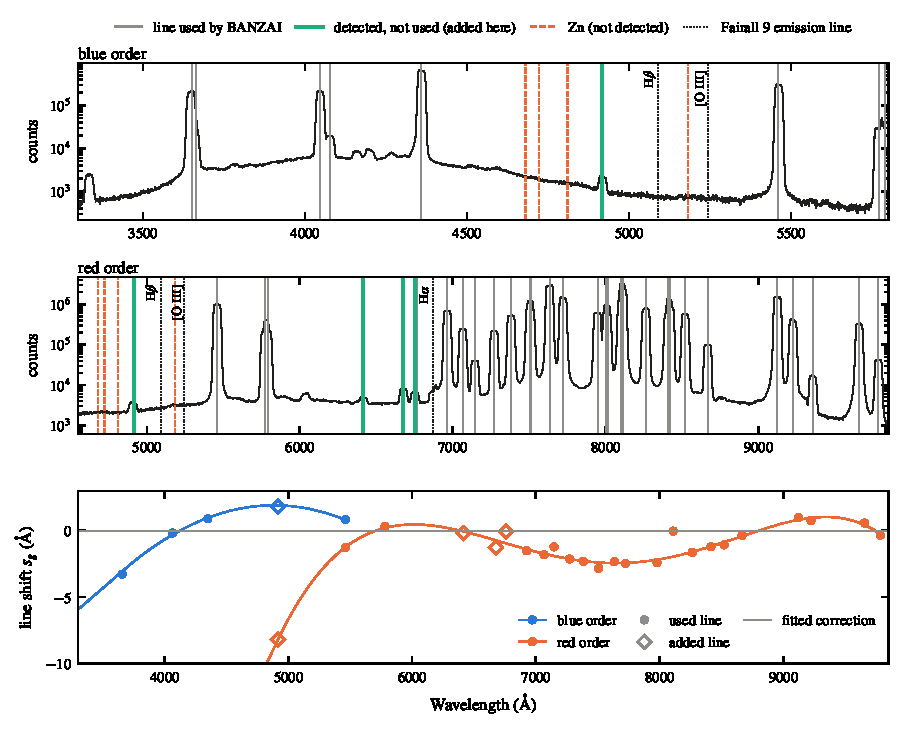
\includegraphics[width=\textwidth]{figures/fig_arcs.pdf}
\caption{Arc lines. Top and middle: one 60\,s arc (6\,arcsec slit) in the blue and red orders. Grey: lines used by
\banzai; aqua: lines detected but not used (Hg\,4916, Ar\,6416, 6677, 6753); dashed orange: Zn lines (lamp ``on''
in the headers, not detected); dotted: H$\beta$, [O\,{\sc iii}] and H$\alpha$ of Fairall~9. Bottom: shift $s_g$ of each
line group (eq.~\ref{eq:arcgroup}) on the \banzai{} solution of 2026-10-08 (circles: used lines; open diamonds: added
lines) and the fitted correction (eq.~\ref{eq:arccorr}). The red order's extrapolated end is off by $-8$\,\AA{} at
Hg\,4916.}
\label{fig:arcs}
\end{figure*}

\begin{figure*}
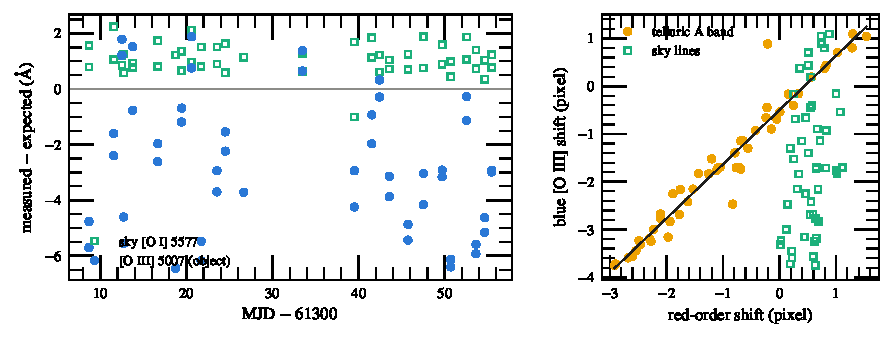
\includegraphics[width=\textwidth]{figures/fig_zeropoint.pdf}
\caption{Left: blue-order [O\,{\sc iii}] shift of Fairall~9 (filled) and 5577\,\AA{} sky-line shift (open) per exposure
in the archive products. Right: blue-order [O\,{\sc iii}] pixel shift against the red-order A-band (filled) and sky-line
(open) pixel shifts; the line has slope 1.13.}
\label{fig:zeropoint}
\end{figure*}

\begin{figure*}
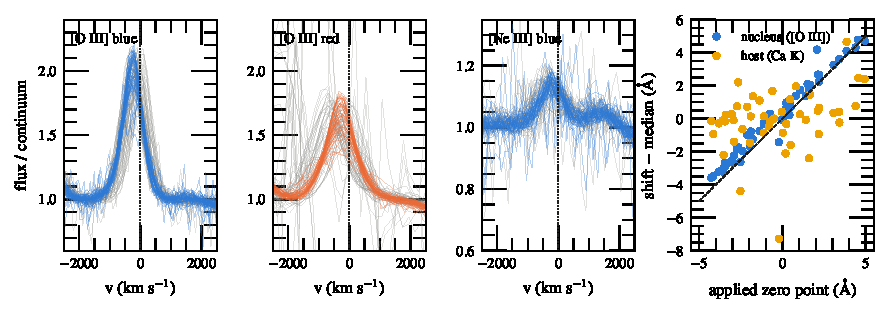
\includegraphics[width=\textwidth]{figures/fig_redshift.pdf}
\caption{Narrow lines of the 50 Fairall~9 spectra in velocity relative to $z=0.047016$: archive (grey) and this work
(colour). Right: shift in the archive products against the applied blue-order zero point for [O\,{\sc iii}] (nucleus)
and Ca\,{\sc ii}\,K (host); dashed: slope 1.}
\label{fig:redshift}
\end{figure*}

\begin{figure*}
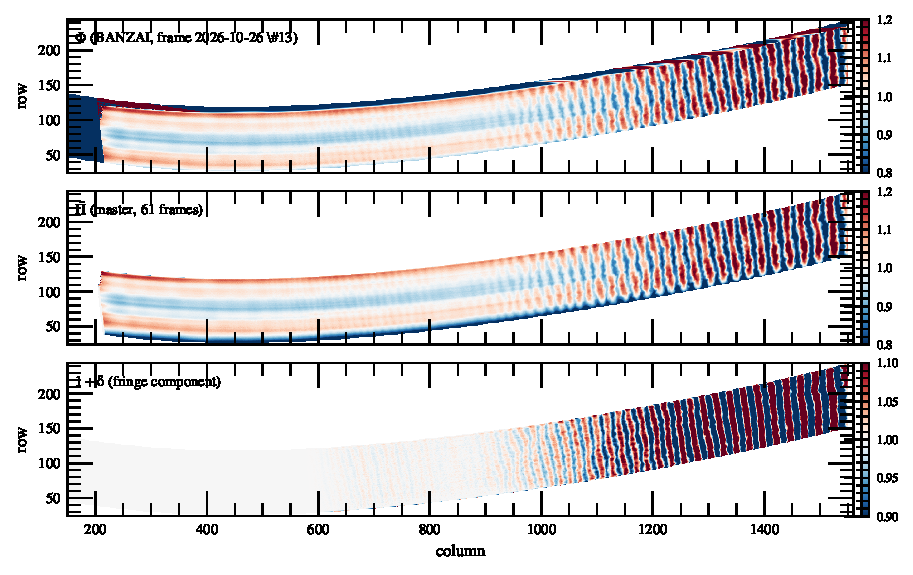
\includegraphics[width=\textwidth]{figures/fig_master.pdf}
\caption{Red order. Top: the map $\Phi$ the archive frame 2026-10-26 \#13 was divided by (shifted by $-8.9$ rows; note
the invalid edges). Middle: the master lamp pattern $\bar\Pi$ from the un-shifted maps of 61 frames. Bottom: its fringe
component $1+\delta$ (eq.~\ref{eq:delta}).}
\label{fig:master}
\end{figure*}

\begin{figure*}
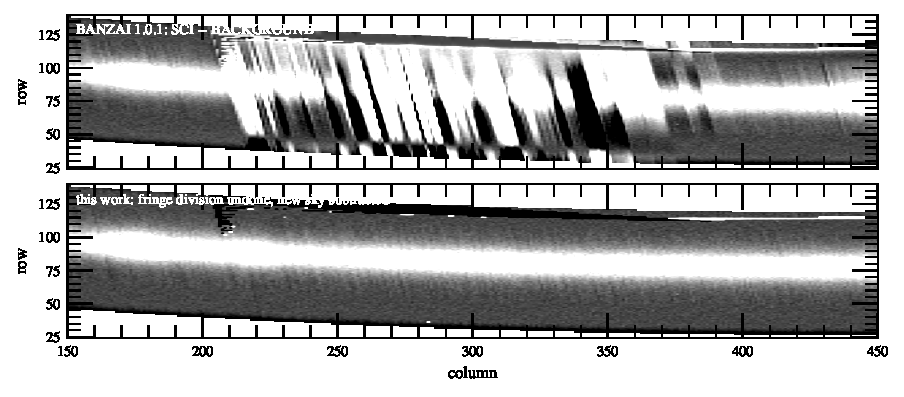
\includegraphics[width=\textwidth]{figures/fig_edge.pdf}
\caption{Red order at $\approx5000$--6000\,\AA{} of the bright-moon frame 2026-10-26 \#13. Top: archive SCI minus
BACKGROUND. Bottom: this work (fringe division undone, invalid pixels masked, new sky subtracted).}
\label{fig:edge}
\end{figure*}

\begin{figure*}
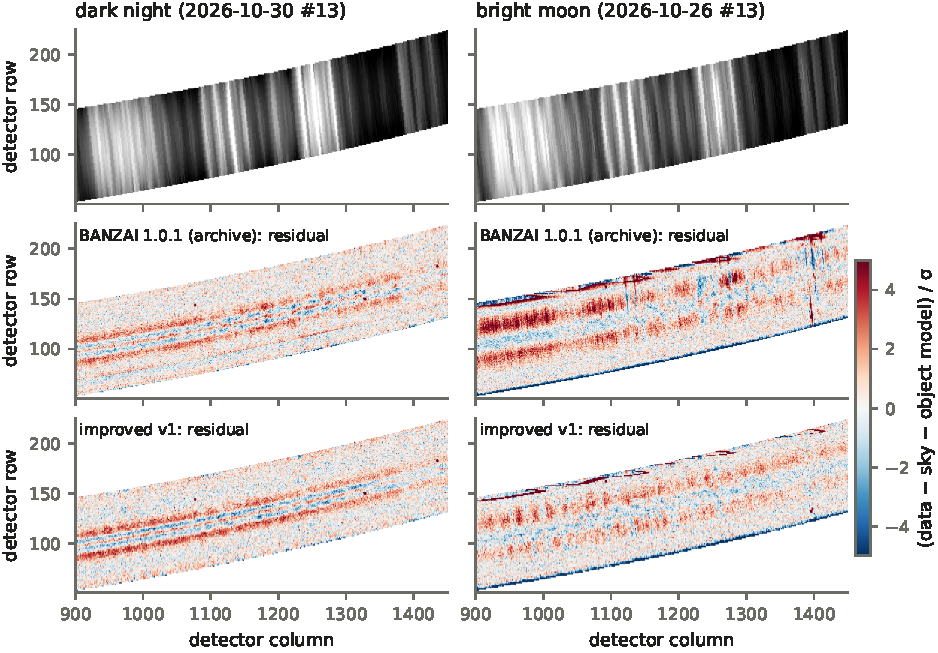
\includegraphics[width=\textwidth]{figures/fig_residuals.pdf}
\caption{Red order at $\approx7600$--9300\,\AA. Top: new sky model. Middle and bottom: normalised residuals (data $-$
sky $-$ profile $\times$ extracted flux)$/\sigma$ of the archive products and of this work, for a dark and a bright-moon
frame.}
\label{fig:residuals}
\end{figure*}

\begin{figure*}
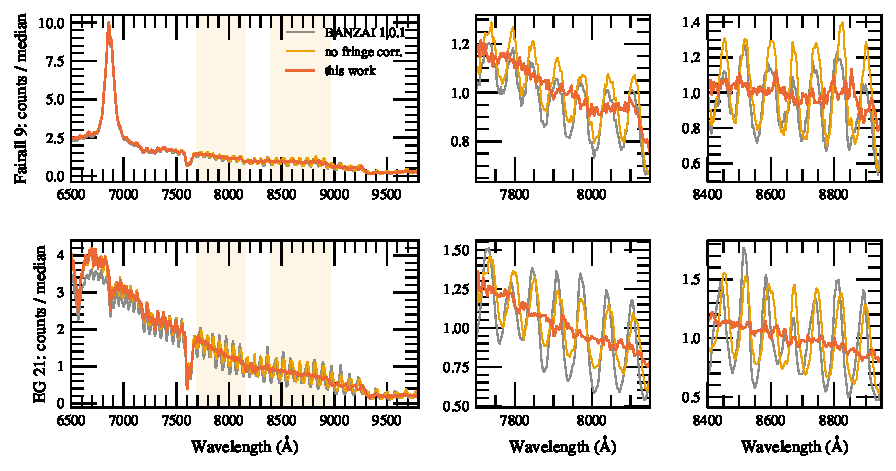
\includegraphics[width=\textwidth]{figures/fig_fringe1d.pdf}
\caption{Extracted red order (counts, normalised) of a Fairall~9 frame and an EG\,21 frame: archive (grey), fringe
division undone without new correction (yellow), this work (orange). The zooms are free of telluric bands.}
\label{fig:fringe1d}
\end{figure*}

\begin{figure*}
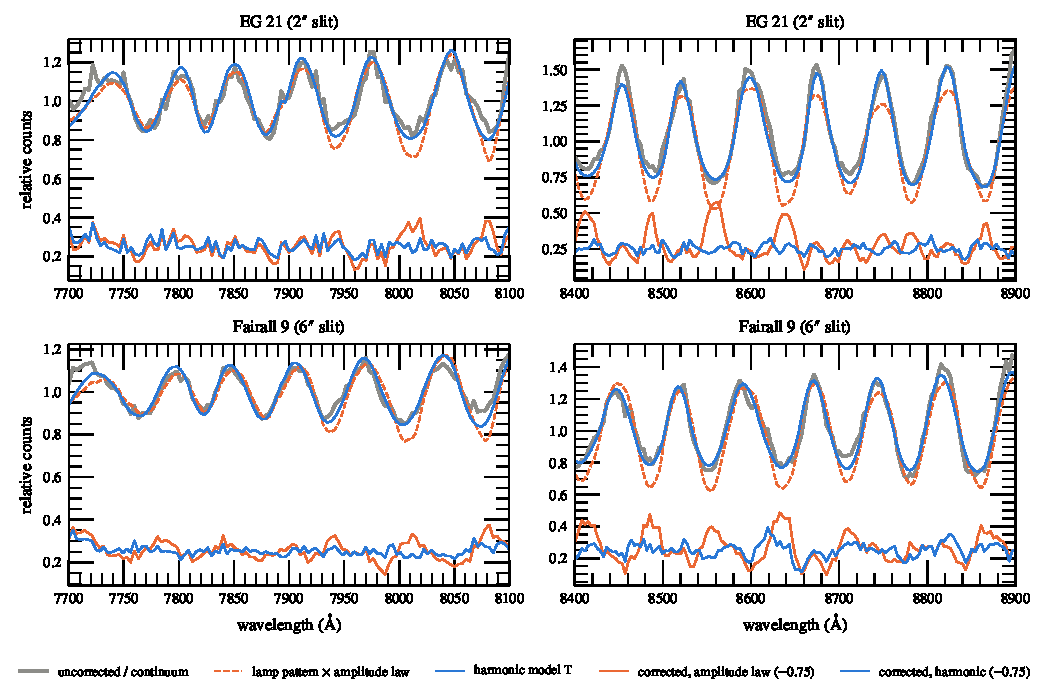
\includegraphics[width=\textwidth]{figures/fig_harmonic.pdf}
\caption{Fringe shape in the red order of an EG\,21 frame (top) and a Fairall~9 frame (bottom), in two windows. Grey:
extraction without fringe correction divided by a 150\,\AA{} running median. Orange dashed: lamp pattern times the
amplitude law (first version); its minima are too deep. Blue: harmonic model $T$ (eq.~\ref{eq:harmonic}). Lower
curves (offset by $-0.75$): corrected spectra divided by their running median.}
\label{fig:harmonic}
\end{figure*}

\begin{figure*}
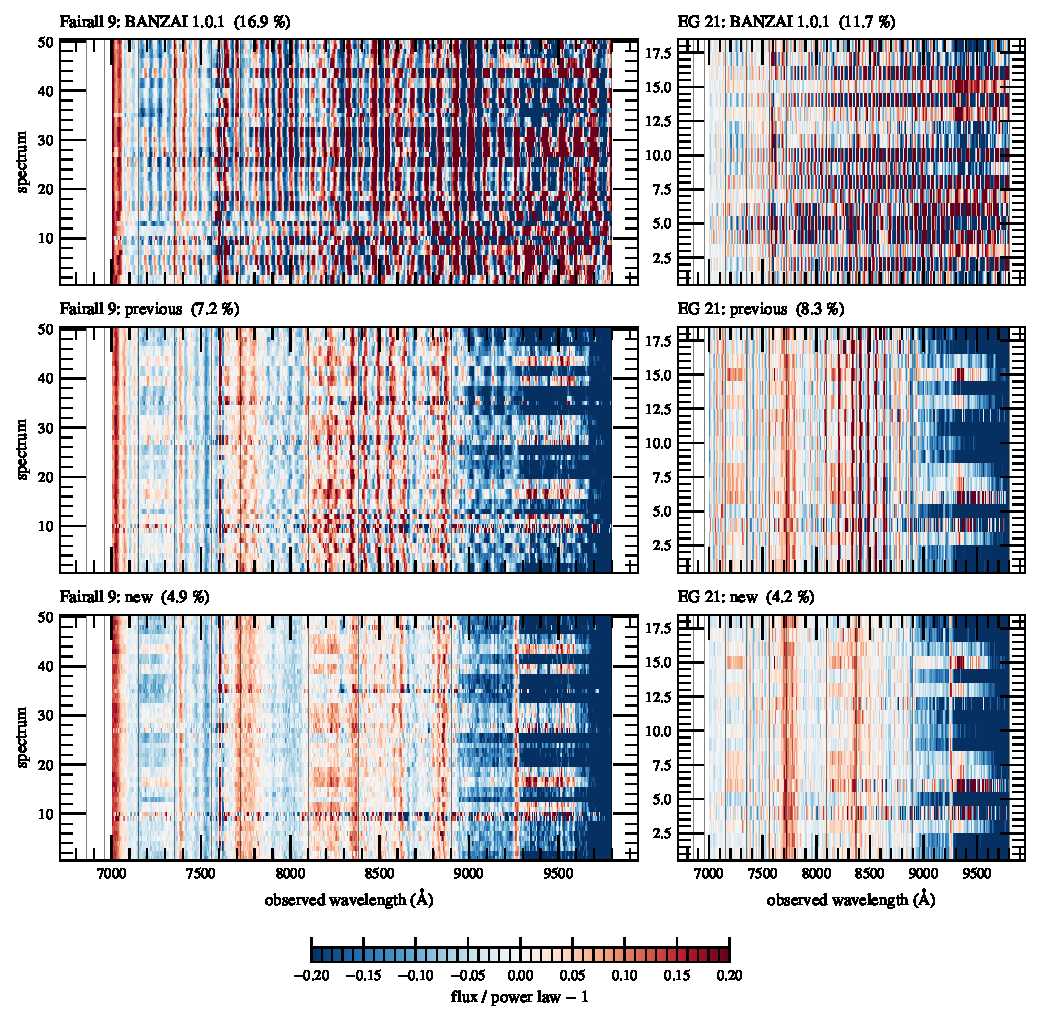
\includegraphics[width=\textwidth]{figures/fig_individual.pdf}
\caption{Individual flux-calibrated red-order spectra (one row per spectrum, in time order) divided by a power law
fitted at 7000--9800\,\AA{} outside the telluric bands (marked by vertical lines). Left: the 50 Fairall~9 spectra;
right: the 18 EG\,21 spectra. Top: \banzai{}~1.0.1; middle: first version of the correction (lamp pattern times
amplitude law); bottom: this work (harmonic model, two passes). The number in each title is the median over spectra of
the rms in 7750--8050 and 8450--8900\,\AA. Remaining vertical structure is common to all spectra (broad lines of
Fairall~9, telluric residuals); horizontal bands beyond 9300\,\AA{} are night-to-night changes of the water-vapour
absorption.}
\label{fig:individual}
\end{figure*}

\begin{figure*}
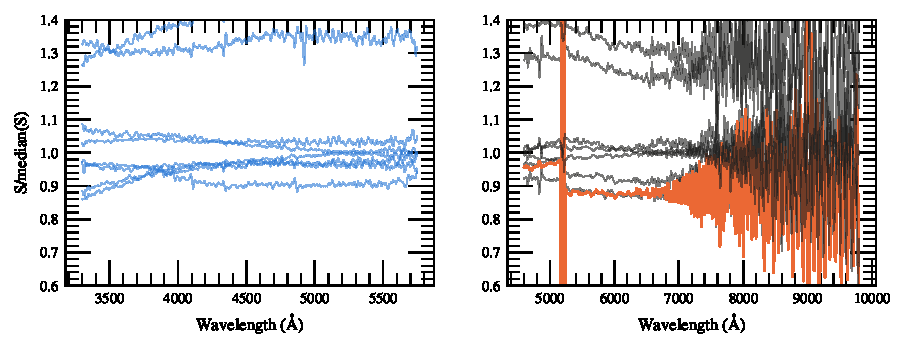
\includegraphics[width=\textwidth]{figures/fig_sens.pdf}
\caption{The eight sensitivity functions used by the archive Fairall~9 spectra, each divided by their median. Orange:
the 2026-10-03 standard (spike at 5200\,\AA). Redward of 7000\,\AA{} the fine-knot fit has learned the fringes of
each standard.}
\label{fig:sens}
\end{figure*}

\begin{figure*}
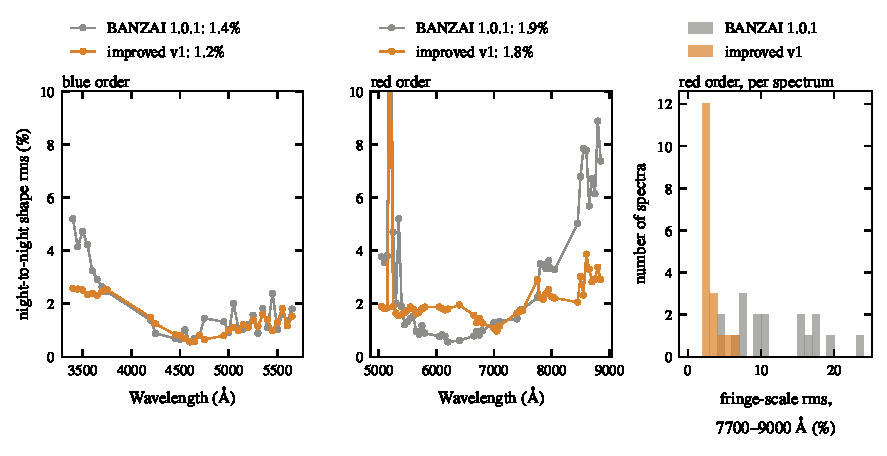
\includegraphics[width=\textwidth]{figures/fig_standard.pdf}
\caption{EG\,21 closure test. Left and middle: night-to-night rms of the shape of the 18 calibrated EG\,21 spectra
relative to the CTIO reference in its 50\,\AA{} bins (telluric and Balmer bins masked): archive (grey) and this work
(each night calibrated with the median sensitivity of the other 17 nights). Right: fringe-scale rms of the red order.}
\label{fig:standard}
\end{figure*}

\begin{figure*}
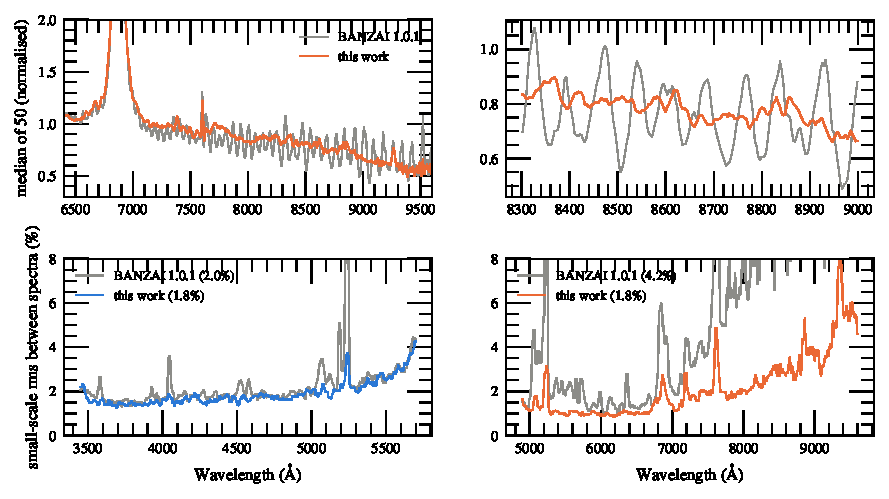
\includegraphics[width=\textwidth]{figures/fig_series.pdf}
\caption{Fairall~9, 50 spectra. Top: median red-order spectrum (left) and a zoom (right). Bottom: small-scale
($<200$\,\AA) scatter between the spectra, blue (left) and red (right) orders; archive in grey.}
\label{fig:series}
\end{figure*}
